\newpage
\part{Sparse Coding}
A signal and its representation are not the same thing. There are an infinite number of possible representation, each capturing different  characteristics of the signal. 

Natural signals have a \emph{sparse representation} in a suitable dictionary due to regularity. Sparsity means that many coefficients vanish, e.g. have zero (or close to zero)  magnitude.
\section{Signal Compression}
Given original signal $x$ and given an orthogonal matrix $A$. Compute the linear transformation (change of basis) $z=Ax$. Truncate "small" values of $z$ which yields an estimate $\hat z$. Compute the inverse transform $\hat x = A^T \hat z$.


The key idea being the \emph{orthogonality} of $A$.

\paragraph{Compressions Algorithm} $\ $
\begin{description}
\item Given an original signal $x$ and an \emph{orthogonal matrix $A$}.
\item Compute the linear transformation (change of basis) $z=Ax$. 
    \subitem Since $A$ is orthogonal, the transformed vector $z$ has the same "energy" as the original signal $x$.
\item Truncate "small" values, giving $\hat z$.
    \subitem We are interested in a \emph{sparse signal}, that is we want $z$ with a small number $K$ of non-zeros.
    \subitem We have compressed the signal since we only need to store $K$ values.
    \subitem The compression is lossy since we have discarded elements of $z$ (by setting them to zero).
\item Compute the inverse transform $\hat x = A^T \hat z$.
    \subitem Since $A^{-1} = A^T$ computing the inverse transform is efficient.
\end{description}

\paragraph{Decomposition and Reconstruction} $\ $
\begin{description}
\item Given a signal $f$ and an orthonormal basis $\{u_1,\ldots, u_L\}$.
\item The coefficients representing signal $f$ in the basis are given by 
    \begin{align*}
        z_l = \langle f, u_l \rangle,
    \end{align*}
    that is $f$ can be reconstructed by
    \begin{align*}
         f=\sum_{l=1}^L z_lu_l = \sum_{l=1}^L \langle f,u_l\rangle u_l.
    \end{align*}
\item Setting certain coefficients $z_l$ to zero is equivalent to not using certain basis functions $u_l$ that is for a subset $\sigma$  of size $K$,
    \begin{align*}
        \hat f = \sum_{k\in \sigma} z_ku_k.
    \end{align*}
\item The reconstruction error is given by
    \begin{align*}
        \norm{f-\hat f}^2 = \sum_{k\notin \sigma} |\langle f,u_k\rangle|^2,
    \end{align*}
    since $\langle u_k, u_l\rangle = 0$ for $k\neq l$.
\end{description}

\subsection{Fourier Basis}
\begin{align*}
 \hat f(\xi) &= \int_{-\infty}^\infty f(x) e^{-2\pi ix\xi} dx & \forall x \in \R\\
 f(x) &= \int_{-\infty}^\infty \hat f(x) e^{2\pi i\xi x}d\xi & \forall x\in \R
\end{align*}

\subsection{Haar Wavelets}
\begin{figure}[H]
\centering
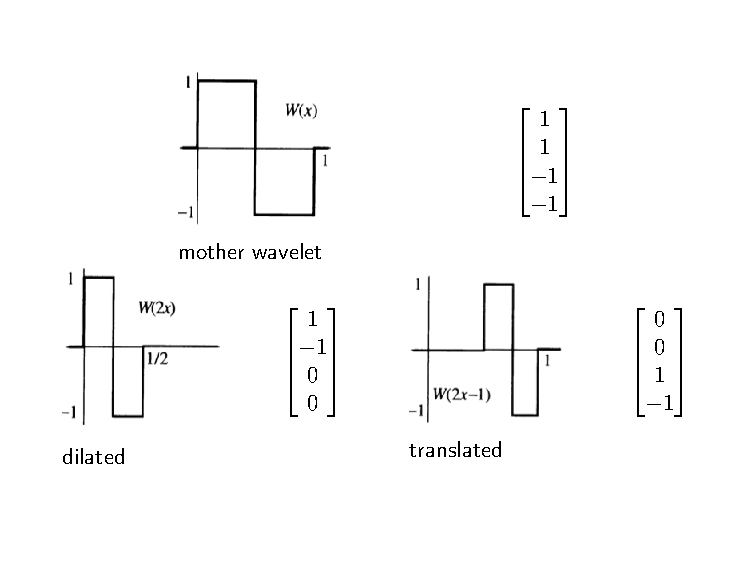
\includegraphics[width=0.7\textwidth]{img/08_haar_wavelets}
\end{figure}


\subsection{Fourier Basis vs Wavelet Basis}
\begin{description}
\item[Fourier Basis] $\ $
    \begin{itemize}
    \item Global support
    \item Good for "sine like" signals
    \item Poor for localised signals
    \end{itemize}
\item[Wavelet Basis] $\ $
    \begin{itemize}
    \item Local support
    \item Good for localised signals
    \item Poor for non-vanishing signals.
    \end{itemize}
\end{description}


\section{Principal Component Analysis (PCA)}
Given $X=[x_1,\ldots, x_N]$ a set of vectors we want to compress. Compute the (centered) covariance matrix:
\begin{align*}
    \Sigma = {1\over N} (X-M)(X-M)^T.
\end{align*}
Compute the eigenvector decomposition:
\begin{align*}
    [U\Lambda] = eig(\Sigma).
\end{align*}
Note that since $\Sigma$ is symmetric $U$ is an orthonormal matrix. Choose $K$ eigenvectors corresponding to the largest eigenvalues $U_K$.

For a given signal $x$ the compressed coefficients are
\begin{align*}
    \hat z = U_K x.
\end{align*}
Also known as the Karhunen-Loeve transform or Hoteling transform.

\subsubsection{Communication Cost}
\begin{description}
\item[PCA Basis] $\ $
    \subitem The basis $U_k$ is dependent on the data and is optimal for the given covariance.
    \subitem Need to transmit both the basis $U$ and the elements of $\hat z$.
\item[Fixed Basis] $\ $
    \subitem Both parties (compressor and decompressor) agree upon a particular basis, e.g. Haar Wavelets.
    \subitem Hence we only need to transmit the non-zero elements of the transformed signal $\hat z$.
\end{description}

\subsection{Compressive Sensing}
Assume that the original signal $x\in \R^D$ is sparse in some orthonormal basis $U$ with $K$ large coefficients in its sparse representation $z$:
\begin{align*}
    x= Uz,\qquad \text{s.t. }|I_{z>>0}| = K.
\end{align*}

The main idea of this method is to acquire the set $y$ of $M$ linear combinations of the initial signal instead of the signal itself and then reconstruct the initial signal from the measured one. 
\begin{align*}
    y_k &= \langle w_k, x\rangle,\ k=1,\ldots,M\\
    y &= Wx = WUz =: \Theta z &\text{with } \Theta = WU \in \R^{M\times D}.
\end{align*}


Surprisingly given any orthonormal basis $U$ we can obtain a stable reconstruction for any $K$-sparse and compressible signal.

This is true under two conditions:
\begin{enumerate}
    \item All elements $w_{i,j}$ of matrix $W$ are i.i.d. random variables with a Gaussian distribution with zero mean and variance ${1\over D}$.
    \item $M:M \geq cK\log\left({D\over K}\right)$, where $c$ is some constant.
\end{enumerate}

To recover the initial signal $x\in \R^D$ from the measured signal $y\in \R^M$ we need to find a sparse representation $z$:
\begin{align*}
    y = Wx = WUz = \Theta z, \qquad \Theta \in \R^{M\times D}.
\end{align*}

Given $z$ we can easily construct $x$:
\begin{align*}
    x = Uz.
\end{align*}

The problem of finding $z$ appears to be \emph{ill-posed} as $M<<D$: Since there are many more unknowns than equations.

Generally this problem is NP hard. Using an approximation scheme like Matching Pursuit is recommended.

\subsection{Sparse Coding}
\begin{description}
\item[Coding via orthogonal transforms] Given original signal $x$ and orthogonal matrix $A$
    \begin{itemize}
        \item Compute linear transformation
            \begin{align*}
                z = Ax
            \end{align*}
        \item Truncate "small" values, giving $\hat z$.
        \item Compute inverse transform (recall $A^{-1} = A^T$)
            \begin{align*}
                \hat x = A^T \hat z
            \end{align*}
    \end{itemize}
\item[Measuring Performance] Sparsity and low reconstruction error.
    \begin{itemize}
        \item Measure the reconstruction error 
            \begin{align*}
                \norm{x-\hat x}.
            \end{align*}
        \item Measure the sparsity of the coding vector $z$ that is $nnz(z)$.
    \end{itemize}
\item[Dictionary Choice] General considereations
    \begin{itemize}
        \item Fourier dictionary is good for "sine like" signals.
        \item Wavelet dictionary is good for localised signals.
    \end{itemize}
\item[Compressive Sensing] $\ $
    \begin{itemize}
        \item Gather and store already compressed signal.
        \item Use $l_0$-norm minimisation to recover initial signal.
    \end{itemize}

\end{description}



























